
\section{Regression}
\subsection{Terminology}

- Data consists of \textbf{pairs} ($\mathbf{x}_n$, $y_n$), where $y_n$ is the n’th output and $x_n$ is a vector of $D$ inputs. The number of pairs $N$ is the data-size and $D$ is the dimensionality.

- Two goals of regression: \textbf{prediction} and \textbf{interpretation}

- The regression function: $y_{n}\approx f_w(\mathbf{x}_{n})\ \forall n$

- Regression finds correlation not a causal relationship.

- \textbf{Input variables} a.k.a. covariates, independent variables, explanatory variables, exogenous variables, predictors, regressors. 

- \textbf{Output variables} a.k.a. target, label, response, outcome, dependent variable, endogenous variables, measured variable, regressands.

\vspace{4pt}
\hrule
\vspace{4pt}
\subsection{Linear Regression}

- Assumes linear relationship between inputs and output.

- $y_{n}\approx\,f(\mathbf{x}_{n}) :=w_{0}+w_{1}x_{n1}+ ... +w_{D}x_{n D} \\ := \tilde{\bf x}_{n}^{T} \tilde{\bf w}$ contain the additional offset term (\small{a.k.a. bias}).

- Given data we learn the weights $\mathbf{w}$ (\small{a.k.a. estimate or fit the model})

- Overparameterisation $D > N$ eg. univariate linear regression with a single data point $y_{1}\approx w_{0}+w_{1}x_{11}$. This makes the task under-determined (no unique solution).

\vspace{4pt}
\hrule
\vspace{4pt}
\subsection{Loss Functions $\mathcal{L}$}

- A loss function (a.k.a. energy, cost, training objective) quantifies how well the model does (how costly its mistakes are).

- $y \in \mathbb{R} \Rightarrow$ desirable for cost to be symmetric around 0 since $\pm$ errors should be penalized equally.

- Cost function should penalize “large” mistakes and “very large” mistakes similarly to be robust to outliars.

- Mean Squared Error: \\ ${\mathsf{MSE}}(\mathbf{w}):={\frac{1}{N}}\sum_{n=1}^{N}\left[y_{n}-f_{\mathrm{w}}(\mathbf{x}_{n})\right]^{2}$ \\ not robust to outliars.

- Mean Absolute Error: \\ ${\mathsf{MAE}}(\mathbf{w}):={\frac{1}{N}}\sum_{n=1}^{N}|y_{n}-f_{\mathrm{w}}(\mathbf{x}_{n})|$

- Convexity: a function is convex iff a line segment between two points on the function’s graph always lies above the function.

- Convexity: a function $h(\mathbf{u}), \mathbf{u} \in \mathbb{R}^D$ is convex if $\forall \ \mathbf{u}, \mathbf{v} \in \mathbb{R}^D, 0 \leq \lambda \leq  1$: \\ $h(\lambda\mathbf{u}+(1-\lambda)\mathbf{v}) \ \textcolor[RGB]{255,0,0}{\leq} \ \lambda h(\mathbf{u})+(1-\lambda)h(\mathbf{v})$ \\Stirctly convex if $\textcolor[RGB]{255,0,0}{\leq} \Rightarrow \textcolor[RGB]{255,0,0}{<}$ 

- Convexity, a desired computational property:
A strictly convex function has a unique global minimum $\mathbf{w^{*}}$. For convex functions, every local minimum is a global minimum.

- Sums of convex functions are also convex $\Rightarrow$ MSE combined with a linear model is convex in $\mathbf{w}$.

- Proof of convexity for MAE:

\scalebox{0.7}{
$\begin{array}{l}
    {\mathsf{MAE}(\mathbf{w}) := \frac{1}{N} \sum_{n=1}^{N} \mathcal{L}_n(\mathbf{w}), \mathcal{L}_n(\mathbf{w})=|y_{n}-f_{\mathrm{w}}(\mathbf{x}_{n})|} 
    \\ 
    {\mathcal{L}_n(\lambda w_1 + (1-\lambda)w_2) \leq \lambda \mathcal{L}_n(w_1)+(1-\lambda)\mathcal{L}_n(w_2)} 
    \\ 
    {| y_n-x_n^{T}(\lambda w_1 + (1-\lambda)w_2)| \leq \lambda |{y_n-x_n^{T}w_1}| + (1-\lambda)|{y_n-x_n^{T}w_2}|}
    \\
    {(1-\lambda) \geq 0 \Rightarrow (1-\lambda)|{y_n-x_n^{T}w_2}|=|(1-\lambda)y_{n}-(1-\lambda)x_{n}^{T}w_2|}
    \\
    {a=\lambda y_{n}-\lambda x_{n}^{T}w_{1}, b=(1-\lambda)y_{n}-(1-\lambda)x_{n}^{T}w_{2}}
    \\
    {a+b=y_{n}-x_{n}^{T}(\lambda w_{1}+(1-\lambda)w_{2})}
    \\
    {|a + b| \leq |a| + |b| \Rightarrow \mathcal{L}_n(\mathbf{w}) \ \mathsf{convex}\Rightarrow \mathsf{MAE}(\mathbf{w}) \ \mathsf{convex}}
\end{array}$
}

- Huber loss: \\
${\cal H}u b e r(e):=\left\{\begin{array}{l l}{{\frac{1}{2}e^{2}}}&{{,\mathrm{if}\ |e|\leq\delta}}\\ {{\delta|e|-\frac{1}{2}\delta^{2}}}&{{,\mathrm{if}\ |e|>\delta}}\end{array}\right.$ convex, differentiable, and robust to outliers but setting $\delta$ is not easy.

- Tukey’s bisquare loss: \\
$\frac{\partial\mathcal{L}}{\partial e}:=\left\{\begin{array}{l l}{{e\{1-e^{2}/\delta^{2}\}^{2}}}&{{,\mathrm{if}\,\,|e|\leq\delta}}\\ {{0}}&{{,\mathrm{if} \ |e| > \delta}}\end{array}\right.$ non-convex, but robust to outliers.

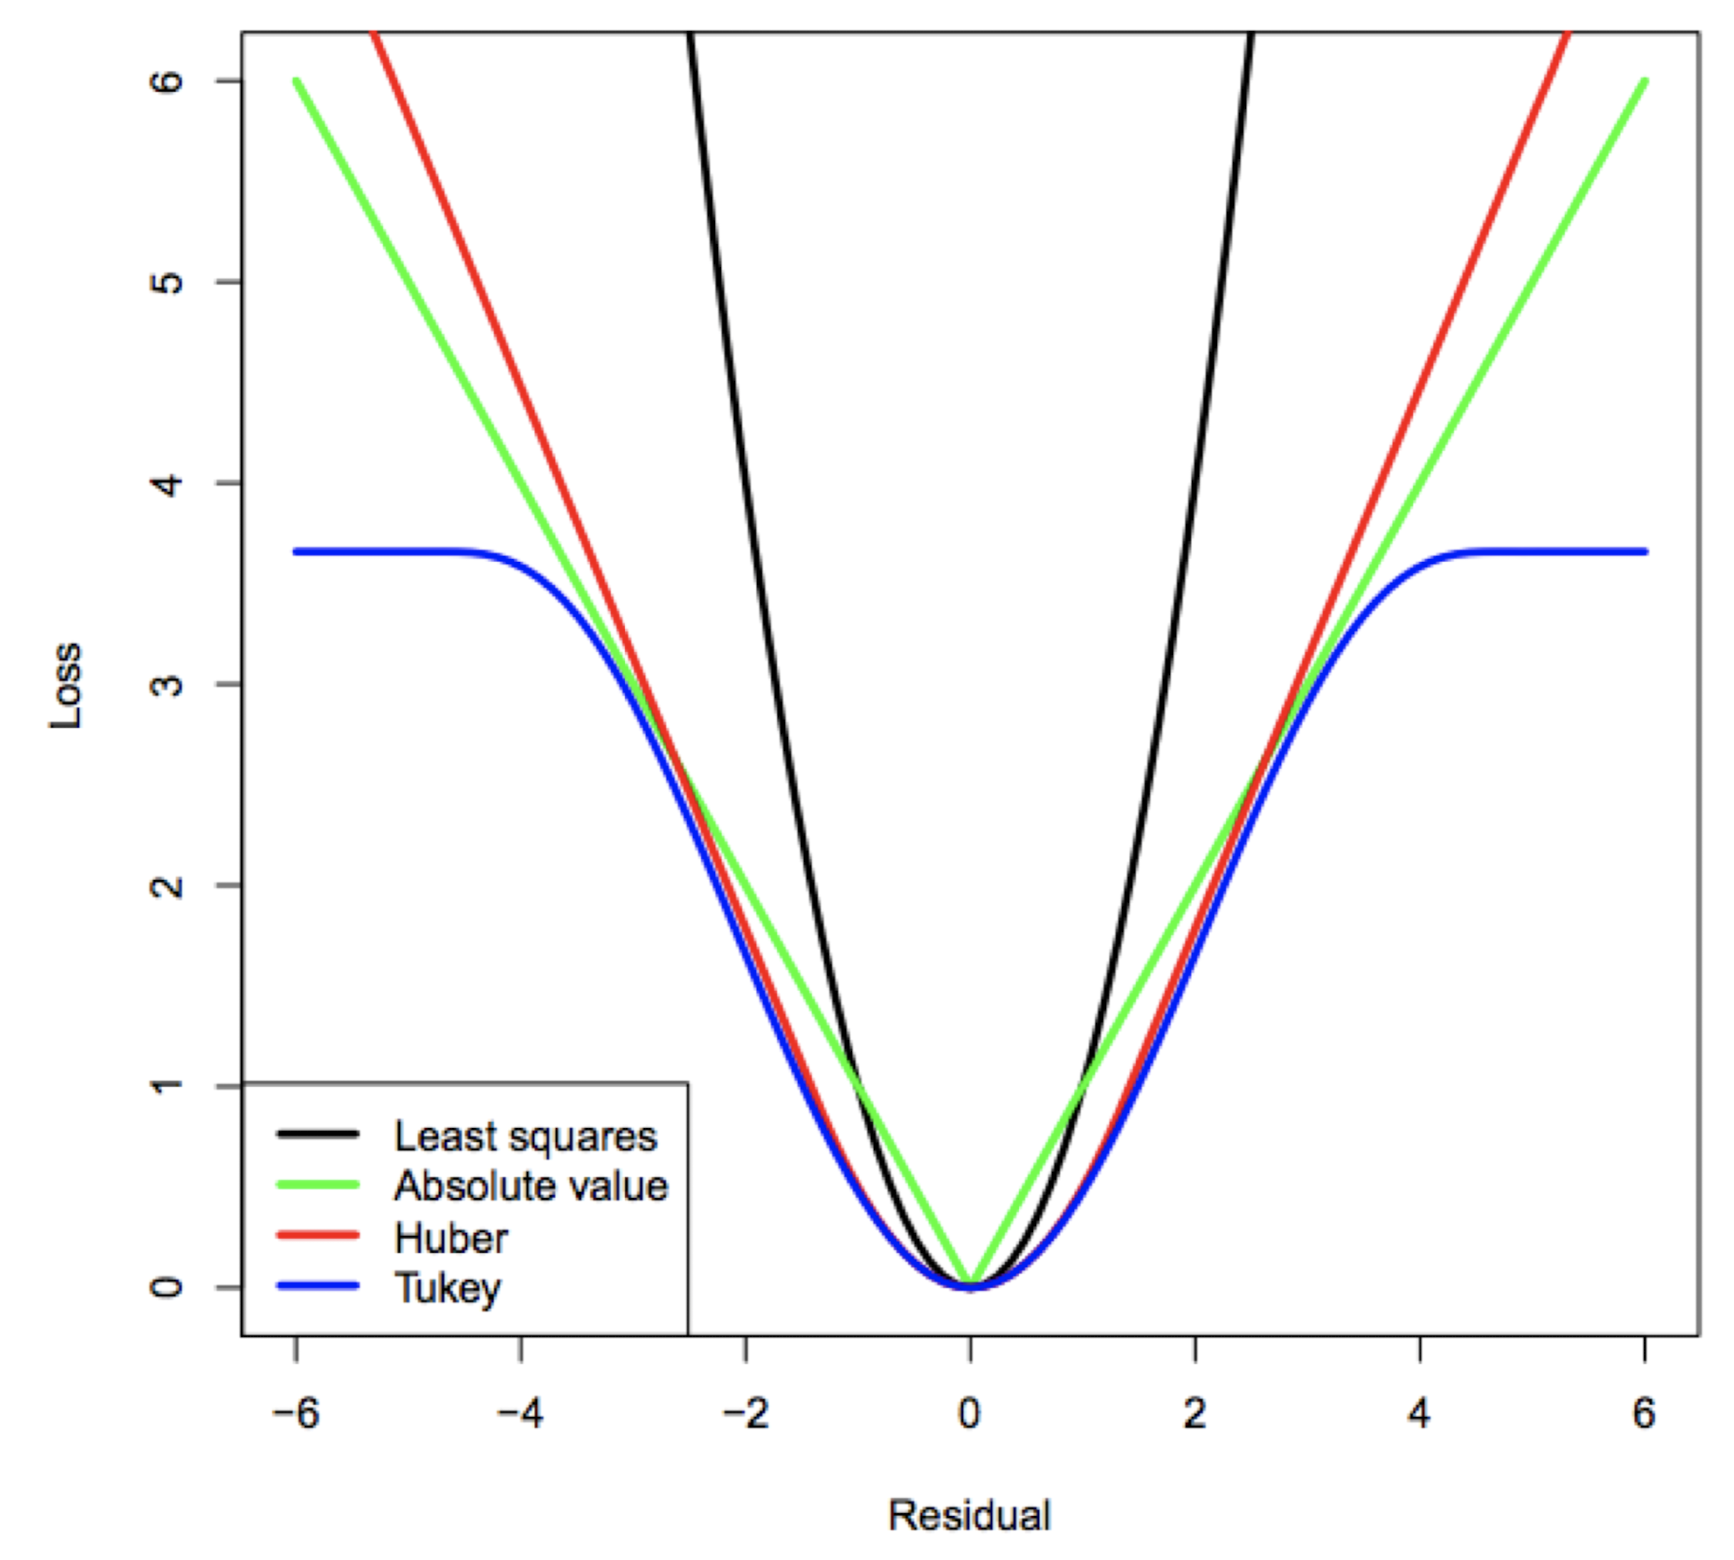
\includegraphics[width=\linewidth]{loss_functions.png}

\vspace{4pt}
\hrule
\vspace{4pt}